\documentclass{beamer}
\usepackage[utf8]{inputenc}
\usepackage[UKenglish]{babel}
\usepackage[UKenglish]{isodate}
\usepackage{tikz}
\usepackage[linesnumbered,ruled,vlined]{algorithm2e}

\usetikzlibrary{arrows.meta}
\usetikzlibrary{backgrounds}
\usetikzlibrary{decorations.pathreplacing}
\usetikzlibrary{fit}
\usetikzlibrary{positioning}
\usetikzlibrary{shapes.misc}

\SetKwFunction{CompileWithBaseCases}{CompileWithBaseCases}
\SetKwFunction{Compile}{{\normalfont \textsc{Crane}}}
\SetKwFunction{Propagate}{Propagate}
\SetKwFunction{FindBaseCases}{FindBaseCases}
\SetKwFunction{Simplify}{Simplify}
\SetKwFunction{Main}{Main}
\SetKwFunction{Input}{ParseCommandLineArguments}

\newcommand{\expr}{\mathtt{expr}}
\newcommand{\Cranetwo}{\textsc{Crane2}}
\newcommand{\Cranebfs}{\textsc{Crane2-BFS}}
\newcommand{\Cranegreedy}{\textsc{Crane2-Greedy}}
\newcommand{\friends}{\emph{Friends \& Smokers}}
\newcommand{\functions}{\emph{Functions}}
\newcommand{\bijections}{\emph{Bijections}}

\beamertemplatenavigationsymbolsempty
\usetheme{default}
\usecolortheme{beaver}

\author{Ananth K. Kidambi\inst{1} \and Guramrit Singh\inst{1} \and \textbf{Paulius Dilkas}\inst{2,3} \and Kuldeep S. Meel\inst{4,2}}
\institute{\inst{1} IIT Bombay, India \and \inst{2} University of Toronto, Canada \and \inst{3} Vector Institute, Canada \and \inst{4} Georgia Tech, USA}

\title{Towards Practical First-Order Model Counting}
\date{SAT 2025}

% TODO: 20 min / 14 slides (presumably)
\begin{document}

\maketitle

% TODO: 2. motivation

% TODO: 3. state the problem

\begin{frame}{Knowledge Compilation Workflow}
  \centering
  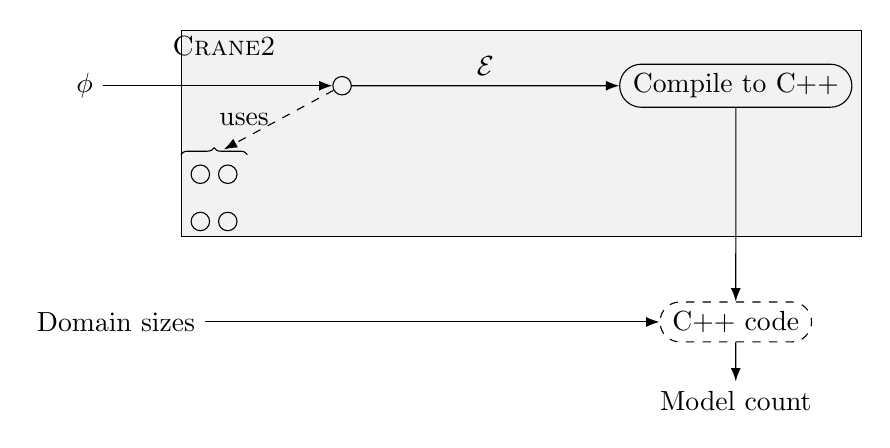
\begin{tikzpicture}
    % Top row
    \node[anchor=west] at (-0.5, 0) (formula) {$\phi$};
    \node[draw,rounded rectangle] at (3, 0) (compilewithbasecases) {\CompileWithBaseCases};
    \node[draw,rounded rectangle] at (8, 0) (compilation) {Compile to C++};

    % Bottom row
    \node[draw,rounded rectangle,dashed] at (8, -3) (cpp) {C++ code};
    \node[anchor=west] at (-1, -3) (sizes) {Domain sizes};
    \node at (8, -4) (count) {Model count};

    % Modules
    \node[draw,rounded rectangle,anchor=north west] at (1.2, -1) (crane) {\Compile};
    \node[draw,rounded rectangle,right=0.1cm of crane] (findbasecases) {\FindBaseCases};
    \node[draw,rounded rectangle,anchor=north west] at (1.2, -1.6) (propagate) {\Propagate};
    \node[draw,rounded rectangle,right=0.1cm of propagate] (simplify) {\Simplify};

    % Bounding box and its name
    \begin{scope}[on background layer]
      \node[draw,fit={(compilewithbasecases) (compilation) (crane) (findbasecases) (propagate)},inner ysep=7pt,yshift=5pt,fill=gray!10] {};
    \end{scope}
    \node at (1.5, 0.5) {\Cranetwo};

    % Brace and its arrow
    \node[fit=(crane)(findbasecases)(propagate)(simplify)] (uses) {};
    \draw[decorate,decoration={brace}] (uses.north west) -- (uses.north east) node[midway] (brace) {};
    \draw[-Latex,dashed] (compilewithbasecases) -- node[midway,left] {uses} (brace);

    % All other arrows
    \draw[-Latex] (formula) -- (compilewithbasecases);
    \draw[-Latex] (compilewithbasecases) -- node[above] {$\mathcal{E}$} (compilation);
    \draw[-Latex] (compilation) -- (cpp);
    \draw[-Latex] (sizes) -- (cpp);
    \draw[-Latex] (cpp) -- (count);
  \end{tikzpicture}
\end{frame}

% TODO: 5. go into detail on the contributions

\begin{frame}{Benchmarks}
  \begin{itemize}
    \item Friends \& Smokers
          \[
          (\forall x,y \in \Delta\text{.
          } S(x) \land F(x, y) \to S(y)) \land (\forall x \in \Delta\text{.
          }S(x) \to C(x))
          \]
    \item Functions
          \begin{gather*}
            (\forall x \in \Gamma\text{. }\exists y \in \Delta\text{. }P(x, y)) \land{}\\
            (\forall x \in \Gamma\text{. }\forall y, z \in \Delta\text{. }P(x, y) \land P(x, z) \to y = z)
          \end{gather*}
    \item Bijections
          \begin{gather*}
            (\forall x \in \Gamma\text{. }\exists y \in \Delta\text{. }P(x, y))\land{}\\
            (\forall y \in \Delta\text{. }\exists x \in \Gamma\text{. }P(x, y))\land{}\\
            (\forall x \in \Gamma\text{. }\forall y, z \in \Delta\text{. }P(x, y) \land P(x, z) \to y = z)\land{}\\
            (\forall x, z \in \Gamma\text{. }\forall y \in \Delta\text{. }P(x, y) \land P(z, y) \to x = z)
          \end{gather*}
  \end{itemize}
\end{frame}

\begin{frame}{Friends \& Smokers}
  \centering
  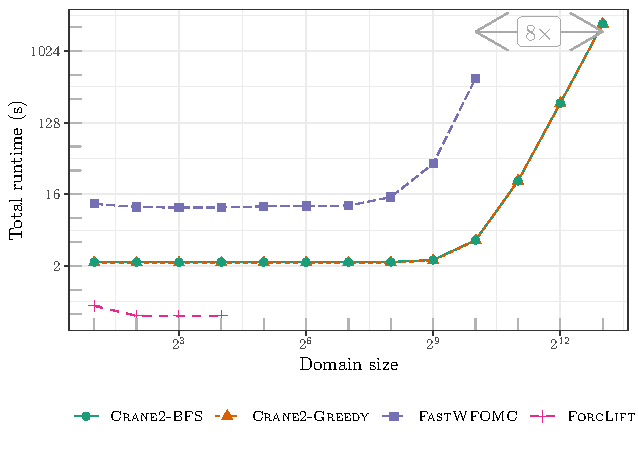
\includegraphics{friends.pdf}
\end{frame}

\begin{frame}{Bijections}
  \centering
  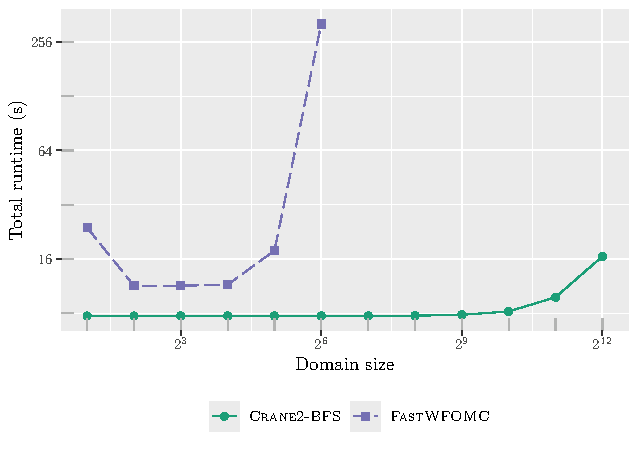
\includegraphics{bijections.pdf}
\end{frame}

\begin{frame}{Functions}
  \centering
  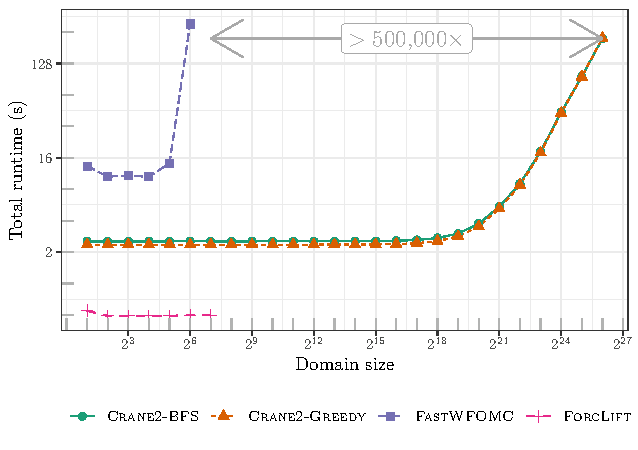
\includegraphics{functions.pdf}
\end{frame}

% TODO: 14. conclusion + future work

\end{document}
